\chapter{Algoritmos para Encaminhamento de Fluxos }%
\label{cap:algoritimos}
Dentre as categorias de atuação das aplicações  de gerenciamento SDN, o presente trabalho está contido na categoria de Engenharia de Tráfego. Com o paradigma SDN, novos requisitos para engenharia de tráfego foram introduzidos utilizando a visão global da rede para desenvolvimento de algoritmos de encaminhamento de fluxo. Esta categoria é importante para otimizar o desempenho da infraestrutura de rede, utilizando análises dinâmicas, predição e regulagem do comportamento da rede~\cite{akyildiz2014roadmap}. Assim é possível maximizar a utilização da rede, minimizar o consumo de energia, efetuar o balanceamento de carga entre outros, permitindo que o administrador tenha maior controle sobre o modo como a rede opera ~\cite{minicurso216}. 

Em infraestruturas com topologias de múltiplos caminhos, as aplicações de gerenciamento de tráfego pode utilizar os dados sobre a rede e efetuar a execução de diferentes estratégias para políticas de encaminhamento de fluxo.
Com isso o presente Capítulo é dividido em: na Seção \ref{sec:encaminhamento} é feito uma revisão sobre encaminhamento de fluxos. A Seção \ref{sec:rr} contém o funcionamento em detalhes da política de encaminhamento \textit{Round-Robin}~(RR), que utiliza múltiplos caminhos para o gerenciamento de rotas. A Seção~\ref{sec:rf} explica o funcionamento da política Caminho Mais Curto Reativo (CMCR). A Seção \ref{sec:pf} contém os detalhes de funcionamento da política Caminho Mais Curto Proativo (CMCP). O funcionamento da política de Caminho de Menor Tráfego (CMT) está descrito na Seção \ref{sec:bw}. A Seção~\ref{sec:trabalhos_relacionados} descreve os trabalhos relacionados e a Seção~\ref{sec:consideracoesparcial_cap3} as considerações parciais do Capítulo \ref{cap:algoritimos}.

\section{Encaminhamento de Fluxos}
\label{sec:encaminhamento}

Diferente dos equipamentos de redes tradicionais que faz roteamento baseado em IP, os dispositivos SDN fazem o encaminhamento de pacotes baseados em regras de fluxos. Os equipamentos não tomam nenhuma decisão, apenas aplicam ações de regras contidas nas tabelas de fluxos para encaminhar o pacote à porta correta. Dessa forma os dispositivos de SDN podem escolher qual camada de rede (\textit{e.g.}, L2, L3, L4) utilizará para efetuar o encaminhamento, dando maior liberdade para as aplicações. 

Conforme mencionado na Seção \ref{sec:openflow} quando um fluxo é ao comutador e este não possui nenhuma regra em sua tabela para realizar o encaminhamento, o comutador envia para o plano de controle um pacote de \textit{packet-in}, o controlador analisa o cabeçalho do pacote para efetuar a configuração dos dispositivos. Com os dados apresentados no cabeçalho do \textit{packet-in} junto a visão completa da topologia que representam o plano de dados, o controlador pode determinar qual caminho deve ser utilizado. Nessa escolha existem diferentes requisitos que podem ser considerados, como: caminho mais curto, maior vazão, menor tráfego e menor latência. Esses requisitos são utilizados em balanceamento de carga para plano de dados com múltiplos caminhos.

Ao determinar quais dispositivos virão compor o caminho do fluxo, o controlador  adiciona ou atualiza regras nas tabelas desses dispositivos. Assim, os próximos pacotes correspondentes ao fluxo não precisarão mais consultar o controlador, pois cada dispositivo que receber o pacote já está devidamente configurado. Dessa forma o encaminhamento será feito para todo novo fluxo adicionado mantendo a utilização da rede sempre otimizada, conforme os algoritmos escolhidos para efetuar o encaminhamento~\cite{akyildiz2014roadmap}.


\begin{figure}[htb!]
	\caption{\label{fig:topo_explicacao} SDN com dois caminhos possíveis.} 
	\begin{center}
	    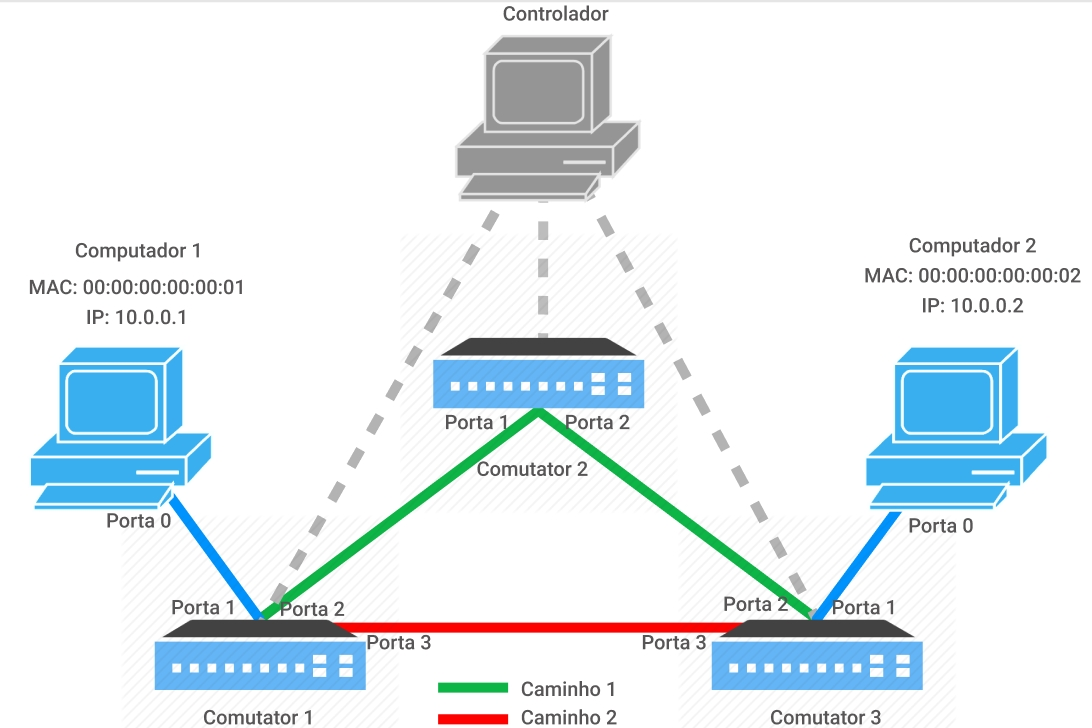
\includegraphics[scale=0.45]{imagens/topologia_explicacao.jpg}
	\end{center}
	\fonte{Elaborada pelo autor (2021).}
\end{figure}

A topologia ilustrada pela Figura \ref{fig:topo_explicacao}  contém dois caminhos possíveis entre o computador 1 e o computador 2. Essa topologia é utilizada para explicar o funcionamento das políticas de RR Seção~\ref{sec:rr}, CMCR Seção~\ref{sec:rf}, CMCP ~\ref{sec:pf} e CMT descrito na Seção~\ref{sec:bw}.

%https://books.google.com.br/books?id=Bc1qAAAAQBAJ&lpg=PT2&ots=nlGoe6R9A6&dq=software%20defined%20networking%20OSPF&lr&hl=pt-BR&pg=PT5#v=twopage&q&f=true

\section{Round-Robin}
\label{sec:rr}
A estratégia do RR é utilizar o algoritmo \emph{First In, First Out} (FIFO) para fazer o escalonamento entre caminhos que podem levar o pacote da origem até o destino, sendo  essa estratégia implementada de forma proativa. O algoritmo faz o balanceamento de novos fluxos criados, fazendo a redistribuição desses fluxos por caminhos alternativos em tempo real, dividindo a sobrecarga dos enlaces. 
Em sua estratégia mais clássica, toda vez que um pacote de um determinado fluxo gera um \textit{packet-in} no comutador, o controlador fica responsável por encontrar todos os caminhos de origem a destino e enfileirar estes caminhos em ordem, de tal forma que o caminho selecionado é removido do início e adicionado ao fim da fila. Este processo é repetido para cada novo \textit{packet-in} gerado, fazendo com que os servidores ao se comunicarem utilizem sempre múltiplos caminhos.

Quando o computador 1 da Figura~\ref{fig:topo_explicacao} executar o comando \textit{ping} ao endereço do computador 2 (\textit{e.g},10.0.0.2), antes de enviar os pacotes de sequência do protocolo ICMP, ele precisa do endereço MAC do destino, para isso é enviado um pacote ARP com MAC destino em \emph{broadcast}. Após a validação do MAC de destino as sequências dos pacotes ICMP começam a ser enviadas. A Figura ~\ref{fig:proxyArp} ilustra o percurso que este ARP realiza na política de RR para a topologia da Figura \ref{fig:topo_explicacao}. O evento 1 do diagrama é o envio do ARP \emph{broadcast} com o endereço MAC de destino ~\emph{FF:FF:FF:FF:FF:FF}. Um \emph{packet-in} é gerado no evento 2 para que o controlador decida a ação. Como o controlador tem a referência do destino é feito um ~\emph{proxy},  procedimento que  entrega o pacote diretamente para o comutador e porta vinculada ao endereço IP do destino, evento 3 e 4, ou possíveis destinos, quando o controlador não tem nenhuma referência conhecida. Nesta topologia, o computador 2 que é o destino, está ligado a porta 1 do comutador 3  . Então o evento 4 do diagrama irá enviar o pacote do \textit{packet-in}, diretamente ao comutador 3 com a ação \textit{output(1)}. O evento 5 ilustra o momento em que o pacote é enviado diretamente ao destino. 

Ao receber o pacote ARP que pergunta qual o MAC do endereço 10.0.0.2, o computador 2 é obrigado a responder com a mensagem \emph{10.0.0.2 at: 00:00:00:00:00:02}, porque este é seu endereço, representado na Figura \ref{fig:proxyArp} pelo evento 6. Caso o ARP entregue pelo controlador não corresponda o endereço, não seria gerado resposta. A resposta entregue ao comutador 3 não possui regras para tratar o pacote, gerando o evento 7 (\emph{packet-in}). Analisando o cabeçalho do pacote o controlador faz novamente o \emph{proxy} entregando diretamente ao comutador 1 para ser enviado pela porta 1 (evento 9 do diagrama). No evento 10 o comutador aplica a ação que veio junto ao pacote, entregando a resposta ao computador 1. Essa forma de resolução de ARP é a mesma para todas as políticas CMCP e CMT. O controlador não insere regra de fluxo durante o processamento de \textit{packet-in} gerado por pacotes ARP, para que o controlador possa comportar dispositivos móveis conectados a pontos de acesso \textit{wireless} de algumas SDN. Dessa forma, para manter a consistência da rede, após um limite de tempo ocioso, a referência que o controlador possui do dispositivo terminal é removida. Nesse caso em que o controlador não tem essa referência, o pacote é enviado para todas as portas que não são enlaces do tipo comutador-comutador, com intuito de encontrar o dispositivo terminal, ou seja, faz uma operação de \emph{proxy}, enviando o pacote para todas as conexões desconhecidas de modo a validar o endereço do computador. Esse formado de resolução de ARP também é útil em redes com múltiplos caminhos, pois entrega os pacotes ~\emph{broadcast} diretamente as portas de comutadores ligados a possíveis dispositivos terminais, evitando futuros \textit{packet-in} para o mesmo pacote. 


%%%%%%%%%%%%%%%%%%%%%%%%%%%%%%____FIGURA__RR___%%%%%%%%%%%%%%%%%%%%%%%%%%%%%%Grafo rede SDN.jpg
\begin{figure}[htb!]
	\caption{\label{fig:proxyArp}Diagrama de sequência, funcionamento da resolução de ARP das abordagens Proativas.} 
	\begin{center}
	    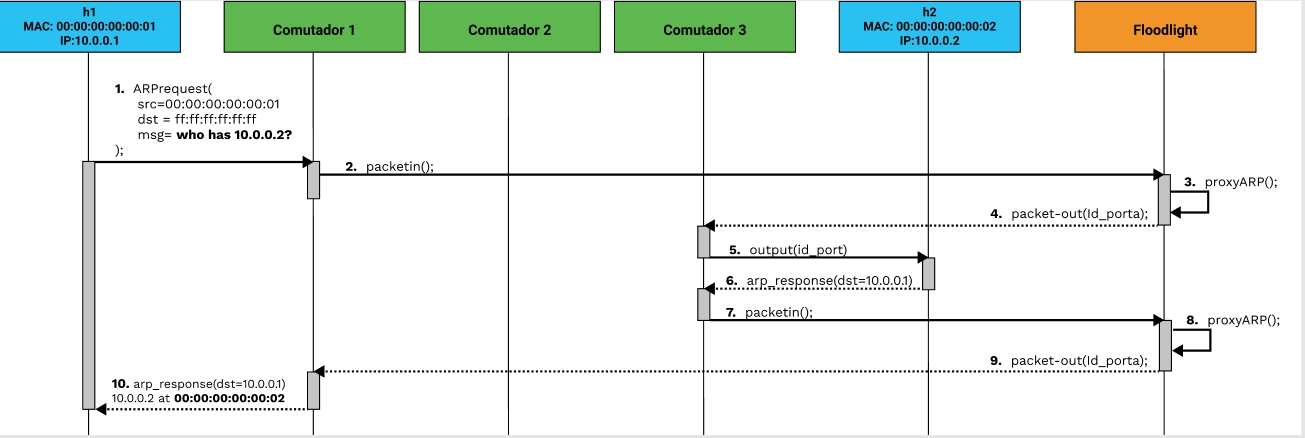
\includegraphics[scale=0.45]{imagens/arpProxy.jpg}
	\end{center}
	\fonte{Elaborada pelo autor (2021).}
\end{figure}

Depois que o ARP é resolvido no evento \textbf{10} do diagrama ilustrado pela Figura \ref{fig:proxyArp}, e o computador que está fazendo a requisição possui a validação do endereço de MAC do destino, então é iniciado o envio das sequências de pacotes. Como o controlador não inseriu nenhuma regra nas tabelas de fluxos dos comutadores, será disparado um \textit{packet-in} já no primeiro pacote. Então é iniciado os eventos começados na sequência \textbf{11} do diagrama da Figura ~\ref{fig:rr}.

\begin{figure}[htb!]
	\caption{\label{fig:rr} Diagrama de sequência, funcionamento da política de ~\emph{Round-Robin}.} 
	\begin{center}
	    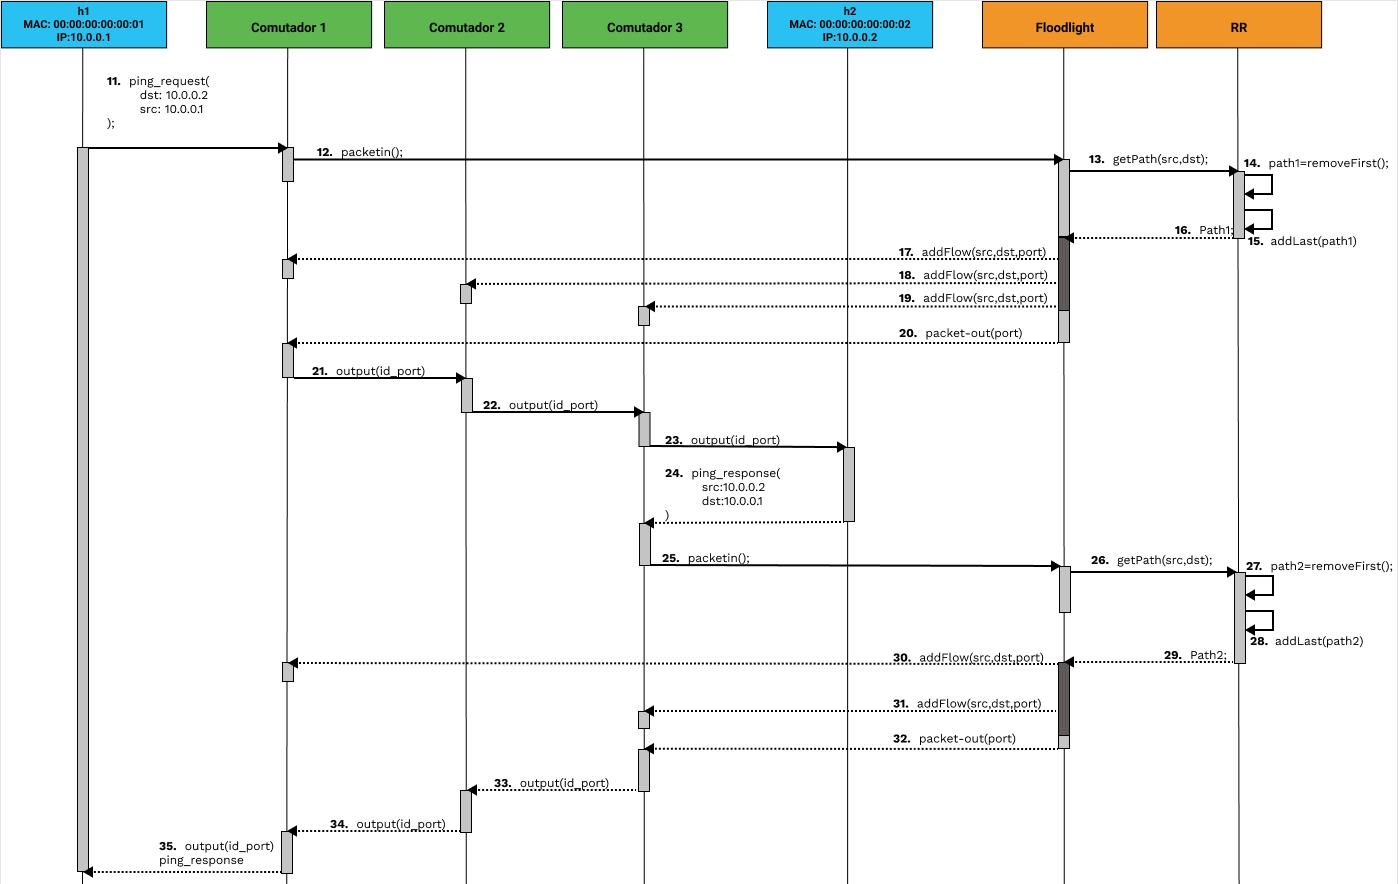
\includegraphics[scale=0.43]{imagens/rr.1.jpg}
	\end{center}
	\fonte{Elaborada pelo autor (2021).}
\end{figure}

O evento 11 é o envio do primeiro pacote ao comutador. No evento 12 o comutador identifica a falta de \emph{match} mara tratar o pacote, gerando um ~\textit{packet-in}. O eventro 13 ocorre com o controlador utilizando os endereços contidos no pacote para buscar o caminho entre origem e destino. Neste cenário  controlador possui dois caminhos enfileirados em um \textit{cache} interno, caminho 1 e caminho 2 da Figura \ref{fig:topo_explicacao}. O evento 14 pega o primeiro caminho nessa fila e o evento 15 passa esse caminho para o fim da fila, a referência do caminho é uma sub lista contendo tuplas de comutador/porta que são necessários configurar para o encaminhamento. 
Como nesse cenário o caminho 1 contém três comutadores, é criado um \emph{match} com as informações do pacote e enviado para o comutador 1, 2 e 3 da Figura \ref{fig:topo_explicacao}, representados no diagrama pelas sequências 17, 18 e 19. O evento 20 ocorre depois da configuração com o controlador devolvendo o pacote recebido no \emph{packet-in} ao comutador que o gerou. Os eventos 21, 22 e 23 são respectivos ao encaminhamento pela aplicação das regras que  determinam a porta de saída. O evento 24 é o momento em que o computador envia a seu comutador a resposta para a sequência 1 do comando \emph{ping}. No evento 25 é gerado outro \textit{packet-in} para tratar a volta do pacote. Passando diretamente ao evento 27, ao selecionar o caminho na fila, o primeiro da lista agora é o caminho 2. O evento 28 passa o caminho 2 ao final da fila e retorna a referência desse caminho contendo o comutador 1 e 3 da Figura \ref{fig:topo_explicacao}. O evento 30 e 31 são acionados para inserção das regras e ações nesses dois comutadores. A última ação do controlador é o evento 32, em que o pacote recebido é devolvido ao comutador que o enviou para seguir seu fluxo configurado. A partir deste ponto, os demais pacotes do fluxo são encaminhados conforme a configuração. Se o fluxo não receber pacotes durante 5 segundos, especificado no contador \textit{idl\_time} o comutador remove o fluxo.


\section{Caminho mais curto reativo}
\label{sec:rf}
A política CMCR faz o encaminhamento pela rota com menor quantidade de comutadores entre origem e destino reativamente, configurando um comutador por vez, ou seja, quando o controlador recebe o \textit{packet-in} ele configura o comutador que o gerou para que o pacote seja encaminhado para o próximo salto. A resolução do ARP nessa política ocorre conforme o diagrama da Figura \ref{fig:rf1}, já os pacotes gerados após a resolução de ARP são ilustrados pela Figura~\ref{fig:rf2}. O cenário utilizado para exemplificar o funcionamento desse algoritmo é o mesmo da Figura \ref{fig:topo_explicacao}.

Antes de iniciar o envio de pacotes da sequência \textit{ping}, o computador 1 precisa do endereço MAC de destino. A forma como a política reativa trata os ARPs \textit{broadcast} é muito similar as redes convencionais. Quando o controlador precisa que um comutador realize um \emph{broadcast}, é adicionado a ação \emph{flood} na construção de um \emph{packet-out}. O \textit{flood} é uma especificação interna do \textit{Openflow}, em que o comutador faz uma cópia do pacote para cada porta de um subconjunto de portas permitidas. Ou seja, portas reservadas, bloqueadas e a porta controlador não são utilizadas na execução do \emph{flood}. 

O primeiro evento ilustrado na Figura \ref{fig:rf1} é o envio da solicitação do endereço MAC do destino. O evento 2 é gerado o \textit{packet-in} pela falta de regras. Como o controlador está utilizando a política de controle de fluxo reativa precisa manter um  \emph{cache} atualizado que contém informações do comutador e os \textit{packet-in} que ele já enviou, para evitar o afogamento dos enlaces gerados em ciclos no plano de dados. Esse controle é representado no evento 3 do diagrama ilustrado pela Figura \ref{fig:rf2}, na qual, o controlador verifica no \textit{cache} do comutador 1 se este pacote já passou uma vez por ele, como é a primeira vez a verificação é falsa, então o pacote é adicionado ao \textit{cache} com o identificador do comutador 1. Após guardar a referência o controlador insere a regra no comutador (evento 6) e devolve o pacote recebido pelo \emph{packet-in} com uma ação \emph{flood}.

\begin{figure}[htb!]
	\caption{\label{fig:rf1} Diagrama de sequência, resolução de ARP na política de encaminhamento reativa.} 
	\begin{center}
	    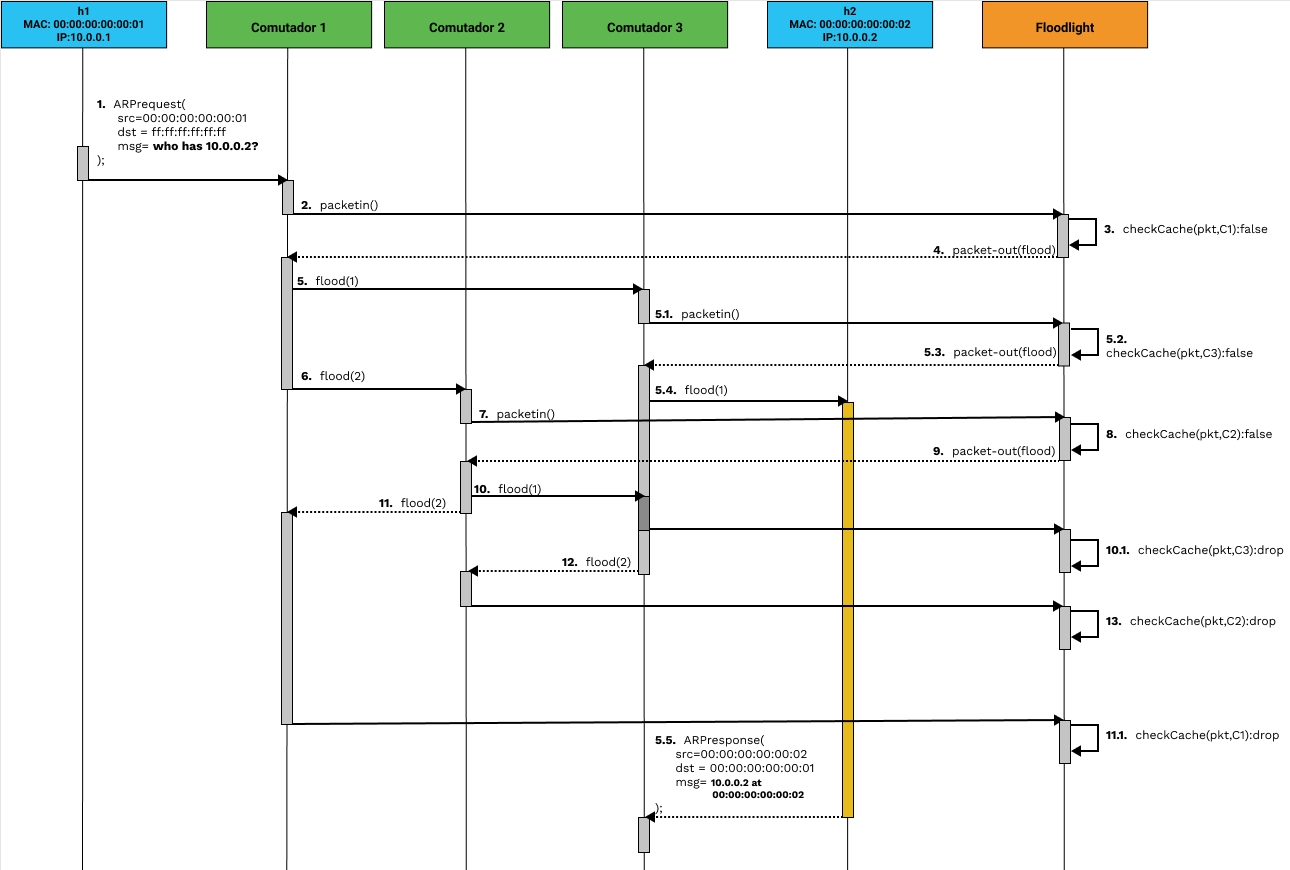
\includegraphics[scale=0.43]{imagens/rf.jpg}
	\end{center}
	\fonte{Elaborada pelo autor (2021).}
\end{figure}

\begin{figure}[htb!]
	\caption{\label{fig:rf2} Diagrama de sequência, funcionamento do caminho mais curto na abordagem reativa.} 
	\begin{center}
	    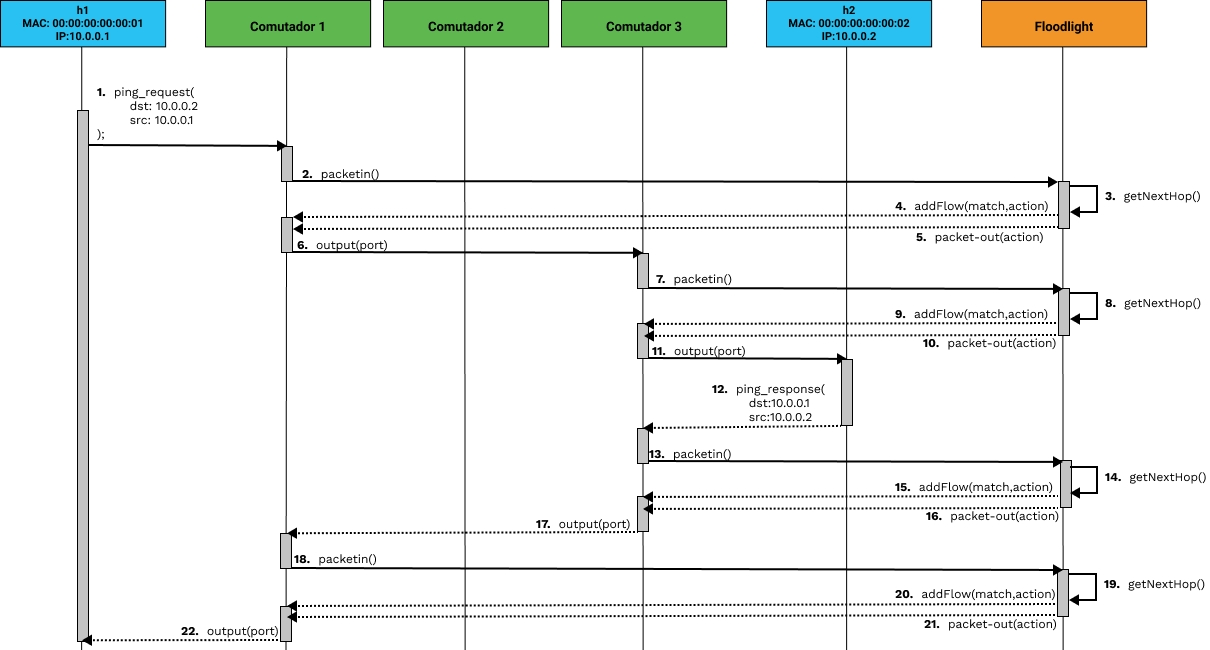
\includegraphics[scale=0.43]{imagens/rf.2.jpg}
	\end{center}
	\fonte{Elaborada pelo autor (2021).}
\end{figure}
Ao processar a instrução \emph{flood} recebida do controlador, o comutador faz a cópia do pacote e o envia para todas as portas válidas, que neste cenário é representada pelos eventos 5 e 6. A partir desse momento o pacote é processado em paralelo pelo comutador 2 e o comutador 3, pois cada um possui uma cópia do pacote.  Os eventos 5.1 e 7 são \emph{packet-in} resultante do recebimento dos pacotes gerados pelo \emph{flood}. O evento 5.2 faz uma verificação do pacote no comutador 3, enquanto o evento 8 realizado em paralelo faz a verificação do pacote no comutador 2. Ambos estão sendo processados pela primeira vez em cada comutador, portanto suas referências são armazenadas no \textit{cache} com a identificação de seus respectivos comutadores. Novamente o controlador irá fazer o \emph{flood} desses pacotes, eventos 5.3 e 9. Quando o comutador 3 realiza a operação de \emph{flood}, uma das portas entrega o pacote ao destino, enquanto a outra porta entrega o pacote ao comutador 2, representado na figura pelo evento 12. 

Quando o controlador analisar o \emph{packet-in} gerado pelo comutador 2 no evento 13, é verificado no \textit{cache} que este pacote já passou uma vez por este comutador, portanto pode ser descartado. Caso esse controle não seja feito, os ciclos no plano de dados clonariam os pacotes indefinidamente. O pacote entregue ao computador pelo evento 5.4 gera a resposta do evento 5.5, assim todo o processo é novamente iniciado para que o pacote volte para origem da requisição. O \textit{cache} do controlador responsável por armazenar a referência dos \textit{packet-in} já processados por cada comutador, possuem um tamanho fixo e as referências mais antigas são descartadas para evitar uso excessivo de memória. 


Após os eventos de pacotes ARP o solicitante envia os pacotes do \emph{ping} com os endereços do destino. A figura \ref{fig:rf2} ilustra o encaminhamento desses pacotes utilizando a política reativa. O evento 1 corresponde ao envio ao comutador, gerando o \emph{packet-in} por falta de regra no evento 2. O controlador busca na topologia interna representada pelo grafo qual o próximo salto do caminho de menor número de saltos, representado pelo evento 3 do diagrama. Como esta política considera apenas um salto, é inserido a regra de fluxo no evento 4 e devolvido o pacote ao comutador no evento 5. O evento 6 representa o encaminhamento para o próximo nó da rede, o comutador 3.
Um novo \emph{packet-in} é gerado no evento 7 repetindo as ações de configuração que consiste em encontrar o próximo salto, configurar o comutador e devolver o pacote, evento 8, 9 e 10. No evento 11 a aplicação da regra sobre o pacote faz a entrega diretamente ao destino. 

O procedimento realizado para o pacote de origem 10.0.0.2 para 10.0.0.1 segue a mesma lógica anterior, eventos de 13 a 22 correspondem a criação de um novo fluxo para que a resposta volte a origem da solicitação. 
%%

\section{Caminho mais curto proativo}
\label{sec:pf}

A política CMCP, utiliza a rota com menor quantidade de saltos entre origem e destino, configurando todos os saltos no primeiro \textit{packet-in}. Considerando o mesmo cenário de exemplo dos algoritmos anteriores, Figura \ref{fig:topo_explicacao}, mesmo que tenha caminhos alternativos o controlador sempre irá escolher o mesmo caminho para criar o fluxo de ida e o fluxo de volta. 

\begin{figure}[htb!]
	\caption{\label{fig:pf} Diagrama de sequência, funcionamento da política de caminho mais curto da abordagem proativa.} 
	\begin{center}
	    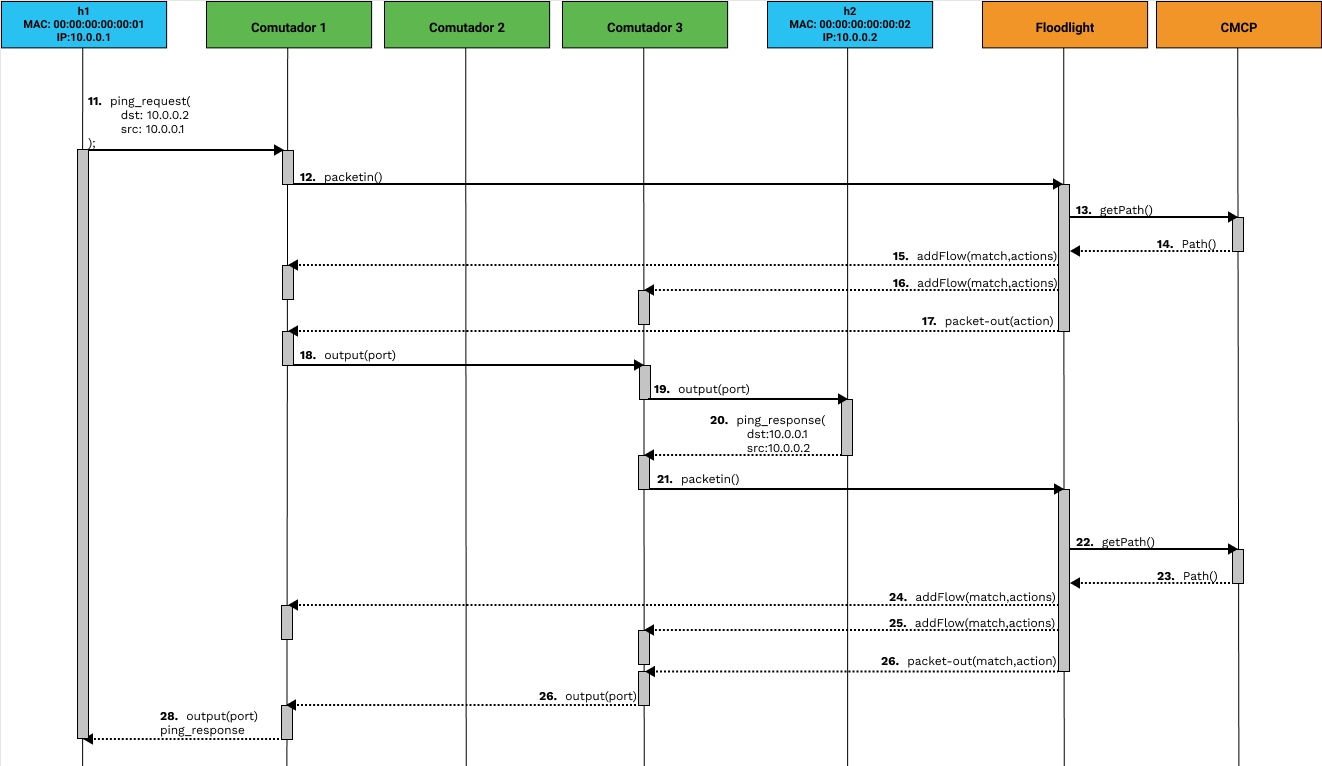
\includegraphics[scale=0.43]{imagens/pf.jpg}
	\end{center}
	\fonte{Elaborada pelo autor (2021).}
\end{figure}
A figura \ref{fig:pf} ilustra o funcionamento da política de encaminhamento para o tráfego gerado pelo comando \emph{ping}. Logo apos os eventos de resolução de ARP usando o \textit{proxy} da Figura \ref{fig:proxyArp}, o próximo evento é iniciado em 11, com a chegada do primeiro pacote da sequência ICMP. Sendo o primeiro pacote o comutador não possui regras em sua tabela para o encaminhamento, gerando o \emph{packet-in} representado na figura pelo evento 12. Ao receber o pacote o controlador faz uma busca no grafo interno que representa a topologia, ilustrado pelo evento 13. Como o grafo tem dois possíveis caminhos, a topologia retorna uma lista ordenada pela quantidade de comutadores em cada caminho, da qual o primeiro da lista é o que possui menor numero de saltos e esta representado pelo evento 14 do diagrama. 

Com as informações de comutadores e portas o controlador gera o \emph{match} com ações para cada elemento do caminho e adiciona essas regras nos comutadores, eventos 15 e 16. Após a inserção das regras o controlador devolve o pacote ao comutador que o enviou junto a uma ação de porta de saída, evento 17. A partir deste ponto o pacote segue o fluxo até o destino, evento 18, 19. 
A resposta gerada pelo destino cria um \emph{packet-in} no evento 21. Como o controlador utilizara novamente o primeiro caminho da lista de caminhos, os comutadores que receberão as regras de fluxo são os mesmos que utilizados anteriormente, eventos 24 e 25. O controlador devolve o pacote no evento 26 para seguir o fluxo,  entregando a resposta do \emph{ping} ao solicitante no evento 28.  
Este algorítimo possui o funcionamento mais simples que os demais, porém utiliza o mesmo caminho mais vezes.



\section{Caminho de menor tráfego}
\label{sec:bw}
Os comutadores que utilizam o protocolo \textit{Openflow} fornecem diversas informações sobre os dispositivos. As informações como bits transmitidos e enviados por cada portas podem ser medias periodicamente para se obter estatísticas como taxa de transferência e assim identificar os enlaces que estão sendo menos utilizados. Tal informação permite a criação de algoritmos que calcula o tráfego de todas as rotas existentes entre origem e destino, assim quando o controlador faz a requisição da rota de menor tráfego esta informação já se encontra pronta para uso.
\begin{figure}[!htb]
	\caption{\label{fig:bw_1}Diagrama de sequência, funcionamento da política de caminho de menor tráfego.}
	\begin{center}
	    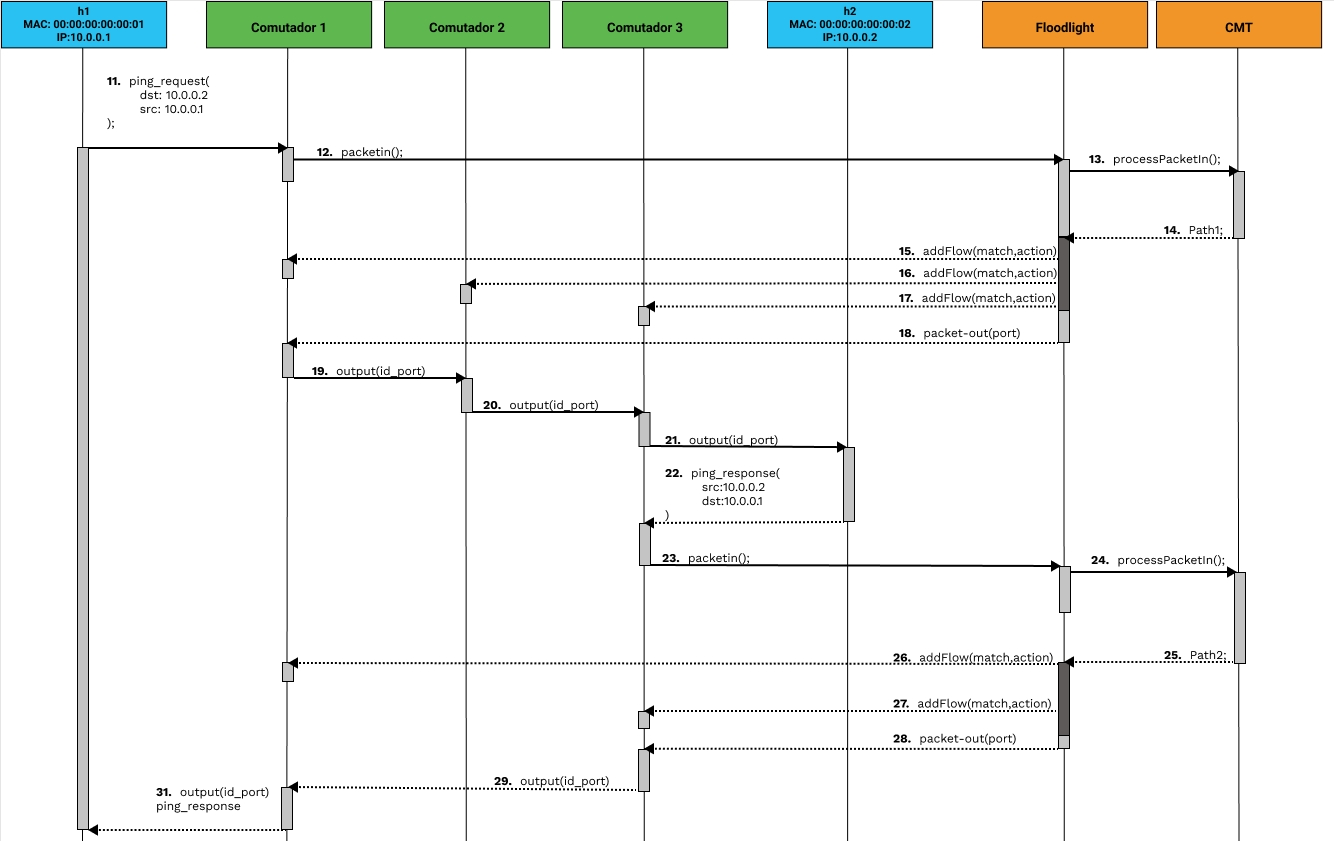
\includegraphics[scale=0.445]{imagens/bw.1.jpg}
	\end{center}
	\fonte{Elaborada pelo autor (2021).}
\end{figure}

\begin{figure}[!htb]
	\caption{\label{fig:bw_2}Diagrama de sequência, troca de informações internas no algoritmo de caminho de menor tráfego.}
	\begin{center}
	    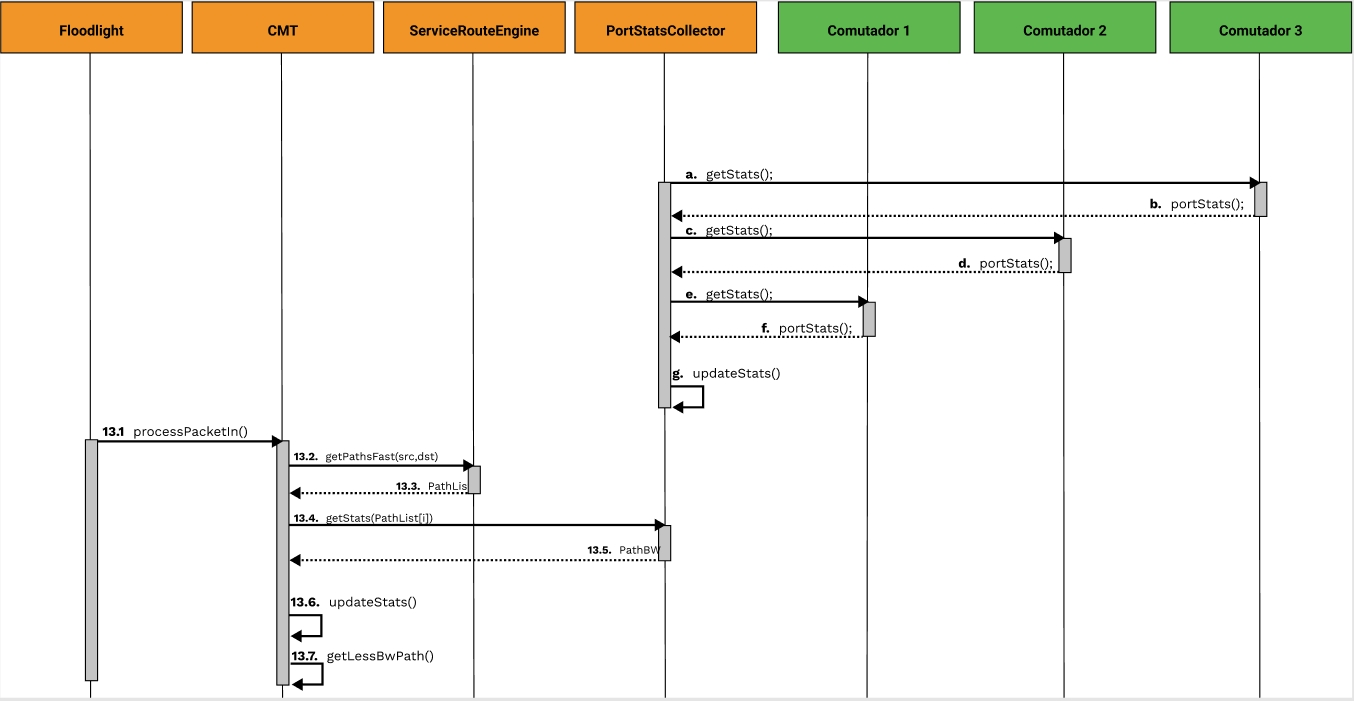
\includegraphics[scale=0.445]{imagens/bw.2.jpg}
	\end{center}
	\fonte{Elaborada pelo autor (2021).}
\end{figure}
A Figura ~\ref{fig:bw_1} ilustra o funcionamento do algoritmo para o envio de um pacote entre ~\textit{~\textbf{h1}} e ~\textit{~\textbf{h2}} com o comando ~\textit{ping} no plano de dados representado pela Figura~\ref{fig:topo_explicacao}. Diferente do algoritmo que considera a quantidade de saltos como caminho mais curto, este utiliza a soma de dados transferidos por cada enlaces do caminho para encontrar qual tem o menor trafego. Caso o caminho 1 que possui maior número de saltos apresente menor utilização de enlaces este é selecionado como caminho de menor tráfego. A vazão total do tráfego é limitado pelo enlace entre o comutador e o computador. Ou seja, se esse enlace é de \textit{1 Gb/s} então mesmo que existam rotas alternativas entre os comutadores não é possível que essa velocidade seja superada.   
O diagrama da Figura ~\ref{fig:bw_1} possui troca de informações divididas em três cores. Em azul estão os computadores, em cor verde os comutadores e em laranja as classes internas do \textit{Floodlight} que foram expandidas na Figura ~\ref{fig:bw_2} com maiores detalhes. Os eventos da figura ~\ref{fig:bw_1} começam na sequência 11 após a resolução de pacotes ARPs, e terminam na sequência 31, com a resposta do comando ~\textit{ping}. Os eventos da Figura ~\ref{fig:bw_2} que vão da sequência 13.1 à 13.7 ocorrem entre os eventos 13 e 14 da Figura ~\ref{fig:bw_1}. 


\begin{table}[!htb]
\centering
\caption{Descrição dos eventos usados para configuração do fluxo na política de menor tráfego.}
\label{tab:bw}
\begin{tabular}{lllll}
\cline{1-2}
\multicolumn{1}{|l|}{\textbf{Evento}} & \multicolumn{1}{l|}{\textbf{Descrição}} &  &  &  \\ \cline{1-2}
\multicolumn{1}{|l|}{11. ping request} & \multicolumn{1}{l|}{\begin{tabular}[c]{@{}l@{}}O primeiro pacote da sequência \textit{ping} já contendo os endereços\\  resolvidos pelo ARP é enviado para o comutador\end{tabular}} &  &  &  \\ \cline{1-2}
\multicolumn{1}{|l|}{12. packetin} & \multicolumn{1}{l|}{\begin{tabular}[c]{@{}l@{}}Como o comutador não possui regra de match para o cabeçalho \\ do pacote, este é enviado ao controlador\end{tabular}} &  &  &  \\ \cline{1-2}
\multicolumn{1}{|l|}{13. processPacketIn} & \multicolumn{1}{l|}{\begin{tabular}[c]{@{}l@{}}O controlador desenpacota a menssagem na qual são extraidas\\  as informações necessárias\end{tabular}} &  &  &  \\ \cline{1-2}
\multicolumn{1}{|l|}{13.2 getPathFast} & \multicolumn{1}{l|}{\begin{tabular}[c]{@{}l@{}}Busca em um grafo/cache local todos os caminhos possíveis \\ entre origem e destino\end{tabular}} &  &  &  \\ \cline{1-2}
\multicolumn{1}{|l|}{13.4 getStats} & \multicolumn{1}{l|}{\begin{tabular}[c]{@{}l@{}}Para cada caminho existente é buscado a soma do trafego entre\\  os enlaces\end{tabular}} &  &  &  \\ \cline{1-2}
\multicolumn{1}{|l|}{13.6 updateStats} & \multicolumn{1}{l|}{A lista é ordenada de forma crecente de tráfego} &  &  &  \\ \cline{1-2}
\multicolumn{1}{|l|}{13.7 getLessBwPath} & \multicolumn{1}{l|}{\begin{tabular}[c]{@{}l@{}}Seleciona o caminho de menor tráfego, gerando uma lista de \\ tuplas com comutador e porta\end{tabular}} &  &  &  \\ \cline{1-2}
\multicolumn{1}{|l|}{15, 16, 17. addFlow} & \multicolumn{1}{l|}{\begin{tabular}[c]{@{}l@{}}É gerado um match com as informações do pacote, cada \\ elemento da lista de tuplas tem sua respectiva ação relacionada a \\ porta de saída. As regras são então enviadas aos comutadores\end{tabular}} &  &  &  \\ \cline{1-2}
\multicolumn{1}{|l|}{18. packet Out} & \multicolumn{1}{l|}{\begin{tabular}[c]{@{}l@{}}Realizado após a adição dos fluxos no switch, devolve o pacote \\ novamente ao comutador que gerou o packet-in para que ele siga\\  o fluxo configurado\end{tabular}} &  &  &  \\ \cline{1-2}
\multicolumn{1}{|l|}{19, 20, 21} & \multicolumn{1}{l|}{\begin{tabular}[c]{@{}l@{}}Comutadores aplicam as ações relacionada ao match instalado\\  anteriormente\end{tabular}} &  &  &  \\ \cline{1-2}
\multicolumn{1}{|l|}{22. ping\_response} & \multicolumn{1}{l|}{O computador de destino envia a resposta para o request} &  &  &  \\ \cline{1-2}
\multicolumn{1}{|l|}{23. packetin} & \multicolumn{1}{l|}{\begin{tabular}[c]{@{}l@{}}Como o controlador configurou apenas a rota de 10.0.0.1 para \\ 10.0.0.2, agora é necessário gerar as regras para tratar pacotes de \\ 10.0.0.2 para 10.0.0.1\end{tabular}} &  &  &  \\ \cline{1-2}
\multicolumn{1}{|l|}{31. ping\_response} & \multicolumn{1}{l|}{A resposta do \textit{ping} é entregue ao solicitante} &  &  &  \\ \cline{1-2}
\cline{1-2}
\multicolumn{1}{|l|}{\textbf{Evento}} & \multicolumn{1}{l|}{\textbf{Descrição}} &  &  &  \\ \cline{1-2}
\multicolumn{1}{|l|}{a,c,e} & \multicolumn{1}{l|}{\begin{tabular}[c]{@{}l@{}}Controlador envia para cada comutador da rede uma solicitação\\  de estatísticas.\end{tabular}} &  &  &  \\ \cline{1-2}
\multicolumn{1}{|l|}{b,d,f} & \multicolumn{1}{l|}{\begin{tabular}[c]{@{}l@{}}Pacotes enviados dos comutadores contendo todas as estatísticas \\ de portas e entradas da tabela de fluxo.\end{tabular}} &  &  &  \\ \cline{1-2}
\multicolumn{1}{|l|}{g} & \multicolumn{1}{l|}{\begin{tabular}[c]{@{}l@{}}As informações são atualizadas em um cache interno para consulta\\  de consumo de comutador/porta\end{tabular}} &  &  &  \\ \cline{1-2}
 &  &  &  &  \\
 &  &  &  & 
\end{tabular}
\fonte{Elaborada pelo autor (2021).}
\end{table}

A Tabela ~\ref{tab:bw} possui uma descrição detalhada sobre os principais eventos que ocorrem para a configuração de um novo fluxo conforme a política de menor tráfego. Sendo que os eventos de ~\textbf{a} até ~\textbf{g} são tarefas paralelas executadas periodicamente a cada segundo, esses são responsáveis por manter a taxa de utilização dos enlaces, calculados e armazenados no \textit{cache} interno do controlador para consultas, de modo a minimizar o tempo de resposta ao \textit{packet-in}. 

\section{Trabalhos Relacionados}
\label{sec:trabalhos_relacionados}
Foram encontrados na literatura seis trabalhos relacionados a avaliação e comparação de políticas de controle de fluxo em SDN. A Tabela \ref{tab:trabalhos_relacionados} traz um levantamento sobre as políticas, métricas de avaliação, topologias e ambientes utilizados para comparação dos algoritmos.

%%%%%%%%%%%%%%%%%%%%%%%%%%%%%%%%%%%%%%%%%%%%%%%%%%%%%
% Please add the following required packages to your document preamble:
% \usepackage{graphicx}
% \usepackage{lscape}
% Please add the following required packages to your document preamble:
% \usepackage{graphicx}
% \usepackage{lscape}
\begin{table}[]
\centering
\caption{Trabalhos relacionados a comparações de políticas de encaminhamento de fluxo.}
\label{tab:trabalhos_relacionados}
\resizebox{\textwidth}{!}{%
\begin{tabular}{lllll}
\hline
\textbf{Referências} &
  \textbf{Algoritmos} &
  \textbf{Métricas} &
  \textbf{Topologia} &
  \textbf{Ambiente} \\ \hline
\cite{akin2019comparison} &
  \begin{tabular}[c]{@{}l@{}}Classe 1:\\ 1. \textit{Minimum Hop Algorithm} (MHA);\\ 2. \textit{Shortest Path}  (SP);\\ 3. \textit{Widest-Shortest Path} (WSP).\\ \\ Classe 2:\\ 1. \textit{Dynamic Shortest Path} (DSP);\\ 2. \textit{Dynamic Widest-Shortest Path} (DWSP).\\ \\ Classe 3:\\ 1. \textit{Minimum Interference Routing}\\ \textit{Algorithm}~(MIRA);\\ 2. \textit{Least Interference}\\ \textit{Optimization Algorithm}~(LIOA);\\ 3. \textit{Improved Least Interference}\\ \textit{Optimization Algorithm}~(ILIOA).\end{tabular} &
  \begin{tabular}[c]{@{}l@{}}1. Total de dados transferidos(\textit{throughput});\\ 2. Quantidade de pacotes perdidos;\\ 3. Tempo de computação do caminho.\end{tabular} &
  \begin{tabular}[c]{@{}l@{}}1. \textit{MIRANET};\\ 2. \textit{ANSNET};\end{tabular} &
  \begin{tabular}[c]{@{}l@{}}Plano de controle: RYU;\\ Plano de dados: \textit{Mininet}.\end{tabular} \\ \hline
\cite{ichikawa2013network} &
  \begin{tabular}[c]{@{}l@{}}1.  \textit{Warshall-Floyd}  (Proposta);\\ 2. \textit{Shortest Path};\end{tabular} &
  \begin{tabular}[c]{@{}l@{}}1. Total de dados transferidos (\textit{Throughput});\\ 2. Tempo de execução do NAS.\end{tabular} &
  \begin{tabular}[c]{@{}l@{}}1. Topologia intra-domínio: \\ (EUA, Japão, Singapura, Tailândia)\end{tabular} &
  \begin{tabular}[c]{@{}l@{}}Plano de controle: Não especificado;\\ Plano de dados: \textit{Open vSwitches}.\end{tabular} \\ \hline
\cite{naeem2020sdn} &
  \begin{tabular}[c]{@{}l@{}}1. \textit{Shortest Path};\\ 2. \textit{Lagrangian relaxation-based}\\ \textit{aggregated cost} (LARAC);\\ 3. Sway;\\ 2. SEQOS baseado \\ em \textit{Bellman–Ford}; (Proposta).\end{tabular} &
  \begin{tabular}[c]{@{}l@{}}1. Custo energético;\\ 2. Total de dados transferidos (\textit{Throughput}).\end{tabular} &
  \begin{tabular}[c]{@{}l@{}}1. \textit{Goodnet};\\ 2. \textit{AttMpls}.\end{tabular} &
  \begin{tabular}[c]{@{}l@{}}Plano de controle:  POX;\\ Plano de dados: \textit{Mininet}.\end{tabular} \\ \hline
\cite{casas2020intelligent} &
  \begin{tabular}[c]{@{}l@{}}1. \textit{Reinforcement Learning and}\\
\textit{Software-Defined Networking} \\ \textit{Intelligent Routing}~(RSIR);\\ 2. Shortest Path (Dijkstra):\\ 2.1. Tráfego;\\ 2.2. Taxa de perda de pacotes;\\ 2.3. Latência;\\ 2.4. Composto (Latencia + Perda + Vazão).\end{tabular} &
  1. Total de dados transferido (Throughput); &
  1. GÉANT: 23 comutadores. &
  \begin{tabular}[c]{@{}l@{}}Plano de controle: Ryu;\\ Plano de dados: Mininet.\end{tabular} \\ \hline
\cite{marcondes2016executing} &
  \begin{tabular}[c]{@{}l@{}}1. Shortest Path;\\ 2. Random Selection;\\ 3. Round-Robin over Multiple Paths;\end{tabular} &
  1. Tempo de execução do NAS. &
  \begin{tabular}[c]{@{}l@{}}1. Fat Tree: 8 servidores e \\ 10 comutadores.\end{tabular} &
  \begin{tabular}[c]{@{}l@{}}Plano de controle: Floodlight;\\ Plano de dados: Mininet.\end{tabular} \\ \hline
\cite{zhang2015performance}&
  \begin{tabular}[c]{@{}l@{}}1. Open Short Path First (OSPF) \\- redes tradicionais;\\ 2. Shortest Path - SDN.\end{tabular} &
  1. Tempo de resposta das requisições. &
  \begin{tabular}[c]{@{}l@{}}1. Topologia de 16 comutadores;\\ 2. Topologia de 120 comutadores.\end{tabular} &
  \begin{tabular}[c]{@{}l@{}}1. Rede tradicional:\\ 1.1. Controle: Quagga;\\ 1.2. Mininext.\\ \\ 2. SDN\\ 2.1. Plano de controle: Floodlight;\\ 2.2. Plano de dados: Mininet.\end{tabular} \\ \hline
\end{tabular}%
}
\fonte{Elaborada pelo autor (2021).}
\end{table}



%%%%%%%%%%%%%%%%%%%%%%%%%%%%%%%%%%%%%%%%%%%%%%%%


Em \cite{akin2019comparison}, foi efetuado um estudo de modo a poder comparar a eficiência entre três classes de algoritmos para controle de fluxo, algoritmos de encaminhamento com: 1) custo de enlace estático, 2) custo do enlace dinâmico e 3) custo do enlace dinâmico com interferência mínima. Na primeira classe contém tês algoritmos de encaminhamento que consideram custo estático como quantidade de saltos. A segunda classe possui duas variações para o caminho mais curto dinâmico, em que é utilizado largura de banda para calcular os pesos de enlaces. A terceira classe contém três algoritmos que adicionam pesos a enlaces criticos junto aos pesos de custo dinâmico. O trabalho comparou essas classes e concluiu que algorítimos dinâmicos tem um desempenho melhor que os estáticos, mas não possuem vantagens significativas entre si dentro de sua própria classe. Em relação à coleta de estatísticas da rede para os algoritmos de custo dinâmico, os autores destacaram duas abordagens. Uma busca manter a projeção atualizada da camada de dados no controlador de modo que o controlador tenha informações o suficiente para identificar os caminhos mais utilizados e estimar largura de banda. A outra abordagem para coleta de informações é fazer leituras periódicas dos comutadores. Esta última abordagem foi utilizada na política de CMT apresentada na Seção \ref{sec:bw}, e os desafios encontrados por este forma leitura são descritos em maiores detalhes na Seção \ref{sec:discussao_resultados}. 

Em \cite{ichikawa2013network} o autor propõe um agente para monitorar informações de latência e vazão permitindo o controlador aplicar no algoritmo de \textit{Warshall-Floyd} e encontrar o melhor caminho. Para validar a proposta o autor utilizou o programa \textit{Numerical Aerodynamic Simulation} (NAS) descrito em detalhes na Seção \ref{sec:aplicacao_teste_nas}. O resultado obtido pelo tempo de execução das aplicações foram comparados com os resultados obtidos pela política de menor caminho e concluiu que a solução proposta teve um desempenho melhor. 

Em \cite{naeem2020sdn}, o autor faz um estudo comparativo entre políticas de controle de fluxo em relação à eficiência do gasto de energia para \textit{Industrial Internet of Things} (IIoT). O autor considera para um bom gerenciamento do tráfego a perda de pacotes, \textit{jitter} e latência em relação ao QoS. O trabalho está relacionado a engenharia de tráfego e demostra como uma decisão tomada no plano de controle pode resolver das mais diferentes categorias de problemas apenas na forma como efetua o gerenciamento. Os resultados do autor mostra que é possível atingir uma redução de até 50\% do custo energético violando apenas 5\% do \textit{Service Level Agreement}~(SLA), resultado aceitável quando se trata de IIoT.

Ainda relacionado a alternativas de algoritmos de encaminhamento, o trabalho de \cite{casas2020intelligent} utiliza roteamento com aprendizagem por reforço como alternativa a gerenciamento do controle de fluxo. A proposta faz leituras periódicas de estatísticas do plano de dados para alimentar um novo plano acima do plano de gerenciamento, chamada \textit{ Knowledge Plane}, que extrai e analisa esses dados gerando o caminho ótimo, na qual, é considerado tanto a largura de banda, perda de pacotes e latência durante a avaliação dos caminhos. Para comparação da proposta o autor utilizou variações do algoritmo de \textit{Dijkstra}~\footnote{Dijkstra é um algoritmo eficiente para encontrar o caminho mais curto em um grafo com pesos em aresta.}, cada uma dessas variações foram baseadas em latência, perda de pacotes, largura de banda e ainda uma versão composta entre latência e largura de banda. A proposta apresentou melhor eficiência ao comparado com o \textit{Dijkstra} latência e \textit{Dijkstra} perda de pacotes, porém teve 3\% a menos de eficiência em relação ao \textit{Dijkstra} com largura de banda.

Em \cite{marcondes2016executing}, o autor compara a política de \textit{Shortest Path} com as políticas de \textit{Random Selection} que escolhe o caminho de forma aleatória, e a política de \textit{Round-Robin over Multiple Paths} cujo funcionamento é baseado em fila circular para escalonamento de caminhos, apresentado na Seção~\ref{sec:rr}. O autor cria uma topologia \textit{Fat Tree} com 8 servidores e 10 comutadores utilizando o \textit{mininet}. Para comparar as políticas utilizou o \textit{framework} NAS e com o tempo de execução das aplicações foi possível identificar que a utilização do \textit{Shortest Path} induz a criação de gargalos na camada de dados. Dessa forma o algoritmo \textit{Round-Robin over Multiple Paths} teve melhores resultados. O desempenho dos algoritmos de múltiplos caminhos são discutidos com mais detalhes na discussão dos resultados Seção \ref{sec:discussao_resultados}.

Em \cite{zhang2015performance}, o autor realiza um estudo entre o protocolo utilizado em redes tradicionais intra-domínio \textit{Open Short Path First}~(OSPF) e a política de encaminhamento padrão do controlador \textit{Floodlight}. Para o estudo o autor criou um ambiente com o \textit{Mininet} e o \textit{Floodlight} emulando uma topologia simples com 16 comutadores e outra topologia mais complexa com 120 comutadores. Para gerar as mesmas topologias na forma de redes tradicionais o autor utilizou o emulador \textit{Mininext}, versão adaptada do \textit{Mininet} para fazer roteamento baseado em \textit{IP} utilizando o protocolo OSPF do \textit{framework} oferecida pelo \textit{Quagga} que é um pacote de programas de roteamento que contém os principais protocolos de roteamento de redes tradicionais. O trabalho utiliza o tempo de resposta gerado pela ferramenta \textit{httping} para comparar os dois cenários. Na qual, conclui que o algoritmo de redes tradicionais possui uma vantagem sobre o de SDN quando o trafego é reduzido, porém, conforme o volume de dados e a escala da topologia é aumentado o protocolo de encaminhamento de fluxo do SDN possui maior vantagem em relação ao tempo de resposta das requisições. O protocolo OSPF utiliza o caminho com menos quantidades de saltos durante o roteamento, esse caminho é calculado durante a inicialização da rede, e seu funcionamento é similar ao funcionamento da política CMCP, assim seu comportamento em relação ao aumento do tráfico também é notável durante a análise dos resultados na Seção~\ref{cap:analise_resultados}.

\section{Considerações Parciais}
\label{sec:consideracoesparcial_cap3}
Neste capítulo foi explicado o funcionamento dos algoritmos de controle e encaminhamento de fluxos comumente utilizados em SDN. 
Dentre políticas existentes citadas na Seção \ref{sec:trabalhos_relacionados} para tratar o encaminhamento de fluxos, foram selecionados apenas duas abordagens baseadas em caminho mais curto, e duas abordagens baseadas em balanceamento de carga para redes de múltiplos caminhos. Nas de caminho mais curto, cujo objetivo é encontrar a rota com menor quantidade de saltos,  uma foi elaborada de forma proativa (CMCP) e outra reativa (CMCR). Para políticas que utilizam balanceamento de tráfego, foi implementado o (RR), que faz o escalonamento entre os caminhos alternativos através de listas circulares. A segunda política de múltiplos caminhos foi (CMT) que usa as informações de \textit{bits} transmitidos por porta oferecidas pelo protocolo \textit{OpenFlow} para determinar o caminho de menor trafego. O Capítulo \ref{cap:protocoleo_experimental} discute a elaboração de uma rede SDN emulada para o estudo do comportamento desses algoritmos apresentados.